\documentclass[11pt,a4paper]{article}
\usepackage[utf8]{inputenc}
\usepackage[margin=2.5cm]{geometry}
\usepackage{amsmath,amssymb}
\usepackage{graphicx}
\usepackage{booktabs}
\usepackage{microtype}
\usepackage[font=small,labelfont=bf]{caption}
\usepackage[numbers,sort&compress]{natbib}
\usepackage[hidelinks]{hyperref}
\usepackage{xurl}
\setlength{\emergencystretch}{3em}
\usepackage{authblk}
\usepackage{setspace}
\setstretch{1.08}

\newcommand{\bits}{\,\mathrm{bits}}

\title{Chess as an Annihilating Boolean Lattice Gas:\\
Survival, Decision Entropy and Irreversibility in Five Classic Games}
\author[1]{Gouri Goutam Borthakur\thanks{Corresponding author: borthakur.gg@gmail.com}}
\affil[1]{Department of Physics, Jorhat Institute of Science and Technology, Jorhat, Assam, India}
\date{}

\begin{document}
\maketitle

%--------------------------------------------------------------------
\begin{abstract}
\noindent
Chess is a finite, fully recorded, rule-complete competition, which makes it a convenient test bed for physical descriptions of decision-driven systems. We model a game as a hard-core lattice gas of two mutually annihilating species: no two pieces share a cell, each piece type carries a hierarchy rank and an existence weight, and a capture is a reaction that releases the victim's weight and marks its cell as a permanent, decision-immune site. The position evolves as a Boolean tensor under XOR updates, and each move is placed in a Boltzmann ensemble of the legal moves, which defines a decision entropy, a surprisal, and an irreversibly accumulated immune information. We implement the model as an open-source Python tool and apply it to five classic games (1858--2013) whose move records were transcribed from two independent sources and verified for legality. Each game is compared with 1000 random-play games and 1000 model-sampled games of equal length. The model yields a consistent set of observables: all five games lose density monotonically, reach immune fractions of 0.26--0.73, show a control field that changes 1.7--2.8 times as many bits per move as the piece field, and show surprisal peaks at sacrificial moves. Only 3 of 60 comparisons with the null ensembles exceed $|z|=3.3$, the decay of decision entropy is largely mechanical, and the sign of the surprisal--entropy gap depends on the ensemble temperature. We discuss what the framework can and cannot establish, and how its three ingredients---exclusion, two opposing species and decision-weighted reactions---map onto ecological, financial and immunological systems.

\medskip
\noindent\textbf{Keywords:} chess; lattice gas; annihilation; Boolean dynamics; decision entropy; survival; irreversibility; statistical physics
\end{abstract}

%--------------------------------------------------------------------
\section{Introduction}

A chess game is one of the best-documented competitive processes there is: finite, governed by a complete rule set, and recorded move by move. It is usually analysed by evaluating positions with an engine, which says who stands better but not what kind of dynamical system a game is. Statistical studies have started to ask the second question. Opening-move frequencies follow a power law whose exponent grows with game depth, and the pooled distribution follows Zipf's law \citep{blasius2009}; move sequences show long-range memory that depends on player skill \citep{schaigorodsky2013}; and engine-based measures of how much each move shifts the expected outcome show skill-dependent decision complexity \citep{chacoma2024}. Regan and Haworth \citep{regan2011} rate players by comparing each move with an engine's evaluation of all legal moves, fitting a sensitivity and a consistency parameter. That construction is close in spirit to the move ensemble used here.

Statistical physics supplies a different and complementary vocabulary. Two species $A$ and $B$ that vanish on meeting, $A+B\to 0$, are a classic problem in reaction kinetics, in which density fluctuations change the decay of the reagents \citep{ovchinnikov1978,toussaint1983}. The same structure appears in finance: the simplest model of Bak, Paczuski and Shubik maps onto diffusing and annihilating particles \citep{bak1997}. Information theory contributes the entropy of a choice among alternatives \citep{shannon1948}, its role in statistical inference \citep{jaynes1957}, and, in Shannon's own proposal for a chess-playing program, the idea of evaluating moves by a numerical score \citep{shannon1950}.

Chess already has the three ingredients of an annihilation lattice gas. Squares are exclusive sites; two opposing species of pieces occupy them; and a capture removes a piece from the board. Mover decisions then determine where and when the reactions happen. What is missing, is a framework that puts exclusion, mutual annihilation, Boolean evolution and decision entropy into one set of observables computed directly from a game record. 
This paper has two aims. The first is to define the model and implement it as a reusable tool. The second is to test, on five classic games and against explicit null ensembles, whether the observables carry information beyond what the rules and the game length already imply. The games serve as a demonstration. The longer-term interest is that the three ingredients are shared by many systems outside chess (Section~\ref{sec:discussion}).

We fixed five hypotheses before running the comparisons:
\begin{itemize}\setlength\itemsep{0pt}
\item[\textbf{H1}] Annihilations cluster in a window in which the number of available captures peaks, and the timing of this window differs between tactical and positional games.
\item[\textbf{H2}] Decision entropy falls over a game, and surprisal exceeds the model entropy at sacrificial moves.
\item[\textbf{H3}] The Boolean control field changes more bits per move than the piece field, and more so in sharp games.
\item[\textbf{H4}] Real games differ from random-play games and from model-sampled games in entropy, immune fraction and related observables.
\item[\textbf{H5}] Survival time by piece type increases with hierarchy rank.
\end{itemize}
Section~\ref{sec:methods} defines the model, data and statistics, Section~\ref{sec:results} reports the results, Section~\ref{sec:discussion} discusses them and Section~\ref{sec:conclusion} concludes.

%--------------------------------------------------------------------
\section{Methods}\label{sec:methods}

\subsection{Lattice gas, species and annihilation}
The $8\times8$ board is a lattice of 64 sites with hard-core exclusion: at most one piece occupies a site, and the code checks this after every ply. White and Black are the two species. Each piece type has a hierarchy rank $h$ (pawn 1, knight 2, bishop 3, rook 4, queen 5, king 6) and an existence weight $w$,
\begin{equation}
w_{\mathrm{P}}=1,\; w_{\mathrm{N}}=3,\; w_{\mathrm{B}}=3.25,\; w_{\mathrm{R}}=5,\; w_{\mathrm{Q}}=9,\; w_{\mathrm{K}}=0 .
\end{equation}
The king has zero weight and is never annihilated; it acts as the absorbing boundary of the game. Each species starts with total weight $W_0=39.5$. The hierarchy rank is used only to order the survival analysis (H5).

A capture is treated as a reaction $W+B\to$ one particle. The victim's weight is released as reaction energy, and the capture cell is marked as a decision-immune site that stays marked for the rest of the game. This is a bookkeeping convention: in chess the capturing piece survives, so the reaction is asymmetric. We keep the convention because it gives a clean conserved quantity, and we return to it in the Discussion. The condensate (immune) fraction is
\begin{equation}
\varphi(t)=\frac{\text{weight released up to ply } t}{2W_0},
\end{equation}
and the surviving weight fraction of a species $\sigma$ is
\begin{equation}
S_\sigma(t)=\frac{\sum_{i\in\sigma,\ \text{alive at } t} w_i}{W_0}.
\end{equation}
Particle density is the number of pieces divided by 64.

\subsection{Boolean evolution}
The position is a Boolean tensor $X_t\in\{0,1\}^{12\times 64}$ (six piece types for each species, 64 sites). A move changes it by an XOR with its difference pattern $D(m_t)$,
\begin{equation}
X_{t+1}=X_t\oplus D(m_t),\qquad A_t=\lVert D(m_t)\rVert_{\mathrm{H}},
\end{equation}
where $\lVert\cdot\rVert_{\mathrm H}$ is the Hamming weight (2 for a quiet move, 3 for a capture, 4 for castling). A second Boolean field $C_t\in\{0,1\}^{2\times64}$ records which sites each side attacks and is updated the same way. The ratio $R_{\mathrm{c/p}}$ of the mean control-field flips per ply to the mean piece-field flips per ply measures how non-locally a single move changes the system.

\subsection{Decision entropy and immune information}
At ply $t$ the mover has $N_t$ legal moves, each with a heuristic energy $s_m$ (in pawn-like units): the weight of a captured piece, a small bonus for central squares and for giving check, and a penalty proportional to the moved piece's weight if it lands on a square attacked by the opponent (larger if the square is undefended). Moves are weighted in a Boltzmann ensemble at inverse temperature $\beta$,
\begin{equation}
p_m=\frac{e^{\beta s_m}}{\sum_{m'}e^{\beta s_{m'}}},\qquad
H_t=-\sum_m p_m\log_2 p_m\le\log_2 N_t,\qquad
I_t=-\log_2 p_{m_t},
\end{equation}
where $H_t$ is the decision entropy and $I_t$ the surprisal of the move actually played. Captures and pawn pushes cannot be undone, so we treat them as ratchets and accumulate their surprisal as immune information,
\begin{equation}
I_{\mathrm{imm}}(t)=\sum_{\tau\le t,\ \text{irreversible}}I_\tau .
\end{equation}
We report the mean entropy $\langle H\rangle$, the entropy drop $\Delta H=\langle H\rangle_{\text{first quarter}}-\langle H\rangle_{\text{last quarter}}$, the gap $\langle I\rangle-\langle H\rangle$ (zero on average for moves sampled from the ensemble itself), and the share $I_{\mathrm{imm}}/\sum I$. Other per-ply observables are the number of available captures $C_t$ (reaction channels), the mixing index (fraction of neighbouring occupied pairs that are unlike) and the number of contested sites. All results use $\beta=1$ unless stated otherwise.

\subsection{Games and data verification}
We analysed five games: Morphy against the Duke of Brunswick and Count Isouard (Paris, 1858); Byrne--Fischer (New York, 1956); Karpov--Kasparov (World Championship, game 16, 1985); Kasparov--Topalov (Wijk aan Zee, 1999); and Aronian--Anand (Wijk aan Zee, 2013). They contrast sacrificial and positional play and span 155 years. For each game, the move list was transcribed from two independent web sources (Section~\ref{sec:data}). The two transcriptions were compared as move sequences, replayed move by move for legality, and checked against the recorded result. All five pairs were identical (33, 82, 80, 87 and 46 plies) and replayed without error; Morphy and Byrne--Fischer end in checkmate and the other three end in resignation.

\subsection{Null ensembles and statistics}
Real games were compared with two ensembles of games of the same length as each real game, started from the initial position and analysed with the same code. \emph{Null A} consists of 1000 games of uniformly random legal moves. \emph{Null B} consists of 1000 games in which each move is drawn from the model ensemble ($\beta=1$). Games that ended before the target length were discarded and replaced. For each observable $x$ and game we report the $z$-score $(x_{\mathrm{real}}-\bar x_{\mathrm{null}})/s_{\mathrm{null}}$. With 6 observables, 5 games and 2 nulls (60 comparisons), we treat $|z|\ge 3.3$ (roughly $p<10^{-3}$ for a normal distribution) as a conservative marker and regard smaller values as descriptive only. Survival order across piece types was assessed by a Spearman rank correlation of the mean final surviving fraction against hierarchy rank.

\subsection{Software}
The model is implemented in Python (\texttt{chess\_physics.py}) using the python-chess library \citep{fiekas2025}, NumPy and Matplotlib. It reads PGN files and writes a text report, a per-ply table and a diagnostic plot per game. The null-ensemble and statistics scripts used here are provided with the code (Section~\ref{sec:data}).

%--------------------------------------------------------------------
\section{Results}\label{sec:results}

\subsection{Observables for the five games}
Table~\ref{tab:games} and Fig.~\ref{fig:games} summarise the baseline run. Density fell monotonically in every game, as it must, from 0.500 to between 0.172 (Kasparov--Topalov) and 0.344 (Aronian--Anand). There were 10 to 21 annihilations, and the immune fraction $\varphi$ ranged from 0.256 to 0.734; in Kasparov--Topalov, 21 captures released 58.0 of the 79.0 units of total weight. The first annihilation occurred between ply 6 and ply 16 (plies 7, 12, 6, 16 and 12 in the order of Table~\ref{tab:games}). The longest chain of captures on one cell was 3 (Morphy and Karpov--Kasparov) and 2 in the other games.

Mean decision entropy was 3.67--4.67 bits against a mean $\log_2 N_t$ of 4.45--5.19 bits. Entropy fell from the first to the last quarter in all five games, by 0.40 to 2.33 bits (Morphy: 4.70 to 2.37 bits). The piece field changed 2.23--2.42 bits per ply on average and the control field 3.9--6.8, so $R_{\mathrm{c/p}}$ was 1.70--2.81. The number of available captures peaked at 5 to 7, at between 0.23 and 0.72 of the game length.

\begin{table}[t]
\centering
\caption{Observables for the five games at $\beta=1$. $\varphi$: immune fraction; $\rho_{\mathrm{end}}$: final density; $\langle H\rangle$ and $\Delta H$ in bits; $R_{\mathrm{c/p}}$: control-to-piece Boolean activity ratio; $C_{\max}$: peak number of available captures and $t_C/T$ its relative position in the game.}\label{tab:games}
\resizebox{\textwidth}{!}{\begin{tabular}{lrrrrrrrrrrr}
\toprule
Game & Plies & Captures & $\varphi$ & $\rho_{\mathrm{end}}$ & $\langle H\rangle$ & $\Delta H$ & $\langle I\rangle-\langle H\rangle$ & $I_{\mathrm{imm}}/\sum I$ & $R_{\mathrm{c/p}}$ & $C_{\max}$ & $t_{C}/T$ \\
\midrule
Morphy--Isouard (1858) & 33 & 12 & 0.487 & 0.312 & 4.09 & 2.33 & 0.12 & 0.40 & 2.81 & 5 & 0.58 \\
Byrne--Fischer (1956) & 82 & 17 & 0.576 & 0.234 & 3.67 & 1.40 & 0.23 & 0.30 & 2.77 & 6 & 0.34 \\
Karpov--Kasparov (1985) & 80 & 17 & 0.554 & 0.234 & 4.53 & 1.71 & 0.11 & 0.37 & 2.09 & 5 & 0.23 \\
Kasparov--Topalov (1999) & 87 & 21 & 0.734 & 0.172 & 3.95 & 1.61 & 0.40 & 0.37 & 2.58 & 7 & 0.72 \\
Aronian--Anand (2013) & 46 & 10 & 0.256 & 0.344 & 4.67 & 0.40 & 0.11 & 0.44 & 1.70 & 7 & 0.54 \\
\bottomrule
\end{tabular}
}
\end{table}

\begin{figure}[t]
\centering
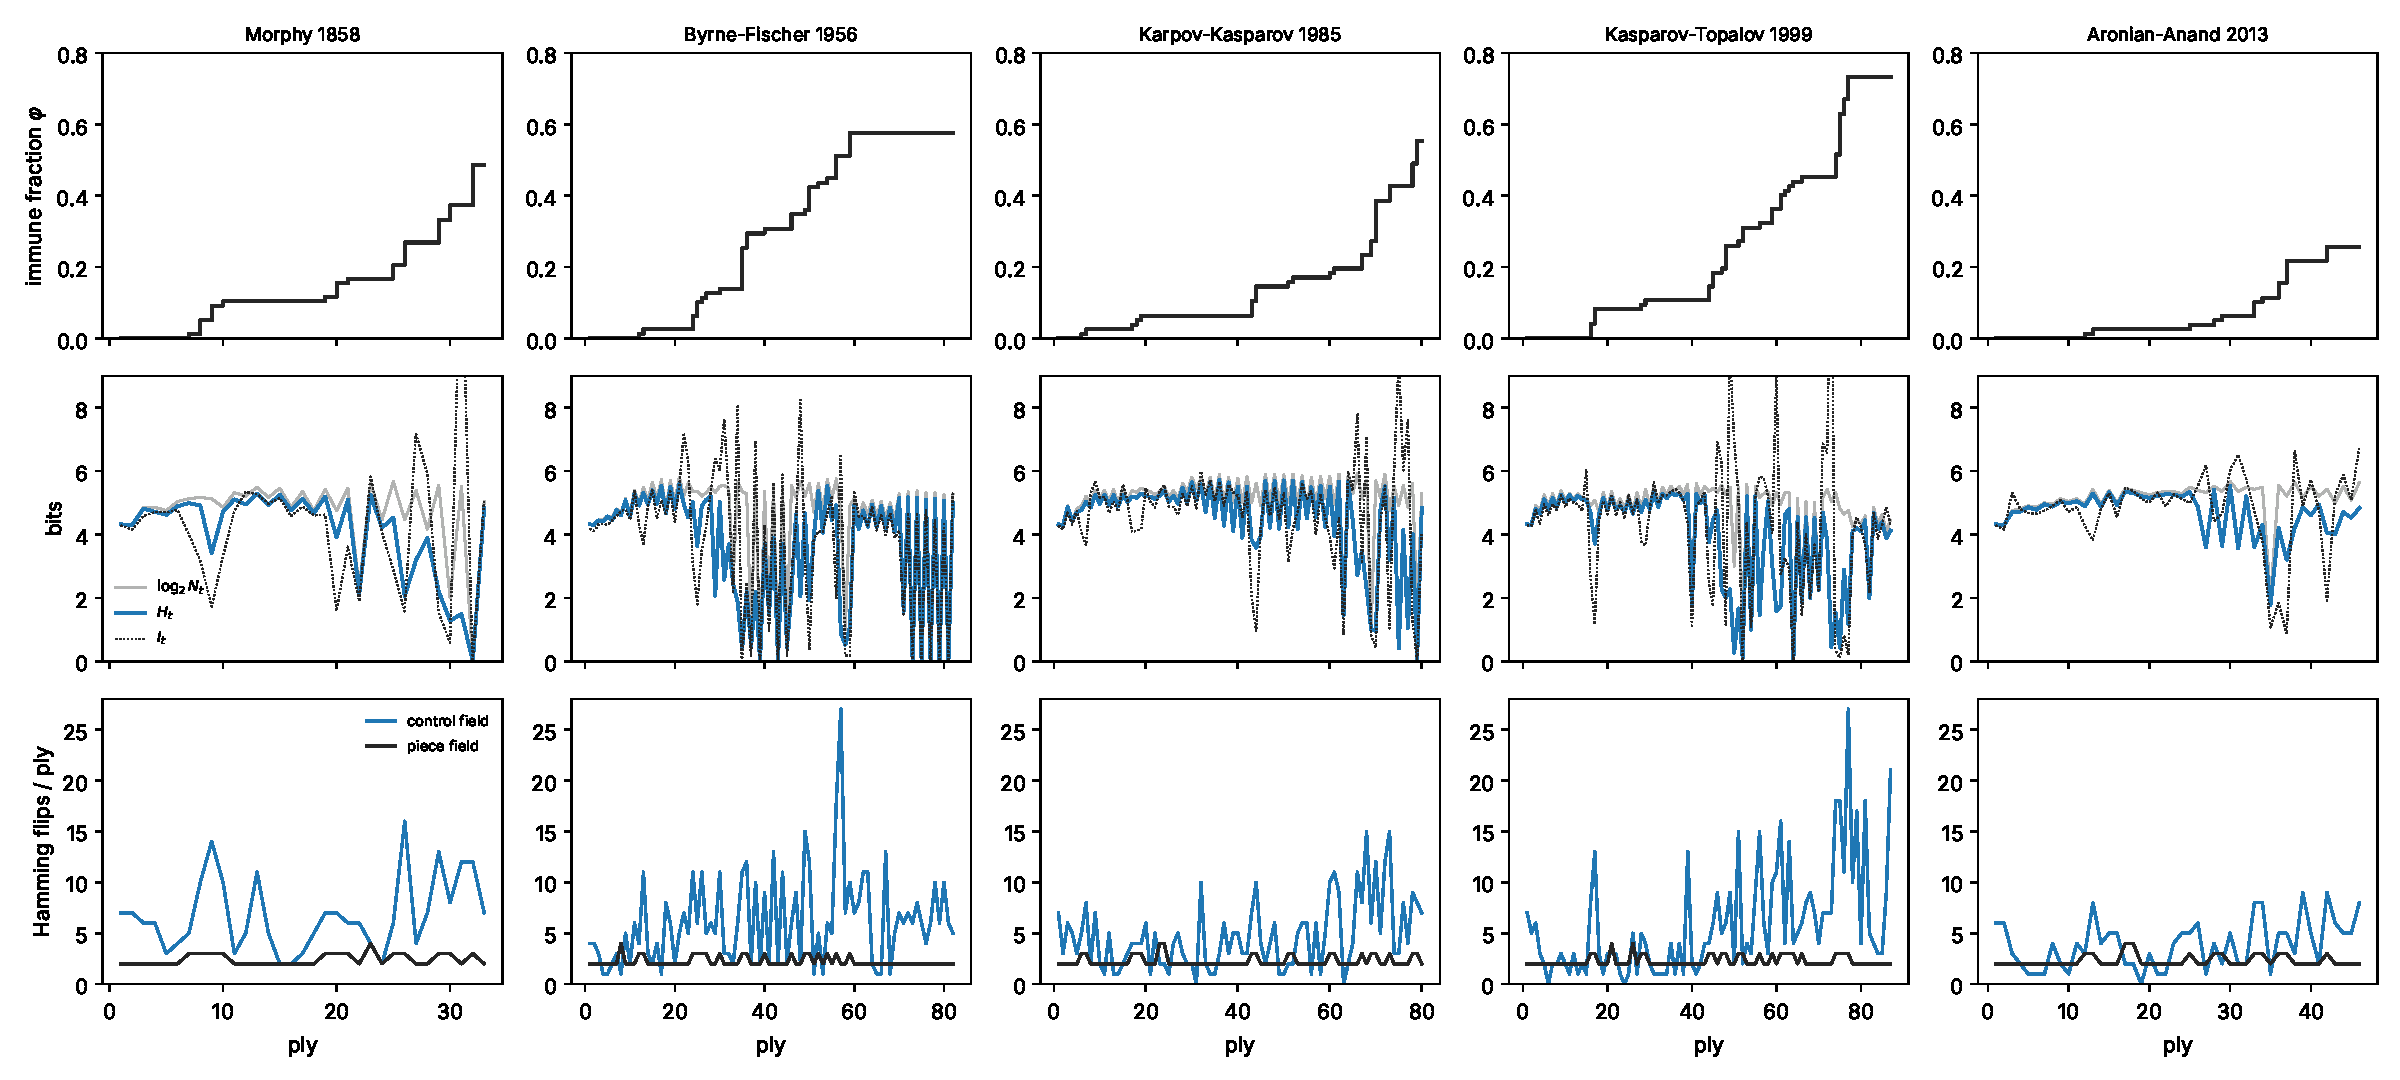
\includegraphics[width=\textwidth]{fig_games.pdf}
\caption{Immune fraction $\varphi(t)$ (top), decision entropy $H_t$, its upper bound $\log_2N_t$ and the surprisal $I_t$ of the played move (middle), and Boolean activity of the control and piece fields (bottom) for the five games.}\label{fig:games}
\end{figure}

\subsection{Survival of the two species}
Figure~\ref{fig:survival} shows the surviving weight fraction of each species. In the three long games (Byrne--Fischer, Karpov--Kasparov, Kasparov--Topalov) both species fell below half of their initial weight within 1 to 5 plies of each other (plies 54 and 59, 78 and 79, 74 and 75), so annihilation was nearly symmetric in time. In Morphy's game only White crossed the half-weight line (ply 32), which reflects a one-sided sacrificial finish; Aronian--Anand ended before either species did. The species with more surviving weight at the end won in only two of five games (Byrne--Fischer, Black, 0.49 against 0.35; Kasparov--Topalov, White, 0.30 against 0.23). Final weights were 0.39/0.64 (White/Black) for Morphy, 0.46/0.43 for Karpov--Kasparov and 0.77/0.72 for Aronian--Anand.

Averaged over the five games, the final surviving fraction was 0.54 for pawns, 0.35 for knights, 0.40 for bishops, 0.45 for rooks and 0.60 for queens. The rank correlation with hierarchy was $\rho=0.40$ ($n=5$ piece types, $p\approx0.5$), so no monotonic ordering can be claimed.

\begin{figure}[t]
\centering
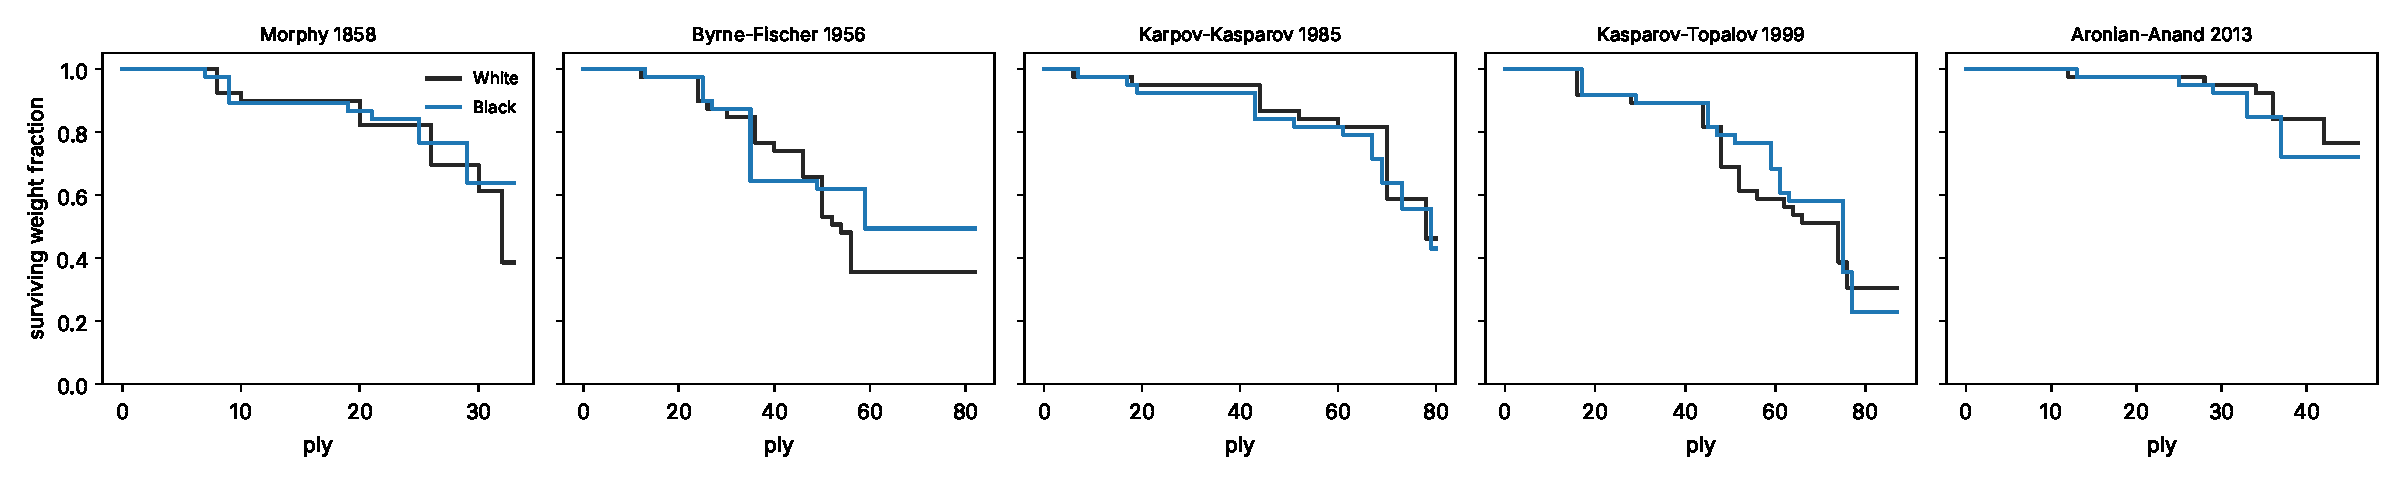
\includegraphics[width=\textwidth]{fig_survival.pdf}
\caption{Surviving weight fraction $S_\sigma(t)$ of White (dark) and Black (blue) in the five games.}\label{fig:survival}
\end{figure}

\subsection{Surprisal at sacrificial moves}
For the four games with a well-known sacrifice we looked at the move itself (Table~\ref{tab:sac}). In Morphy's game, the queen sacrifice 16.Qb8+ had $H_t=1.49$ bits but $I_t=13.68$ bits, the most surprising ply of the game. Fischer's 17\ldots Be6 ($I_t=8.04$, $H_t=1.86$) and Kasparov's 24.Rxd4 ($I_t=6.26$, $H_t=2.29$) ranked at the 98.8th and 94.3rd percentile of $I_t-H_t$ within their games. Anand's 16\ldots Nde5, a knight move in a position with many reasonable options ($H_t=5.21$), reached only the 73.9th percentile ($I_t=5.74$).

\begin{table}[t]
\centering
\caption{Entropy and surprisal at the selected sacrificial move of each game ($\beta=1$). Percentile: share of plies in the same game with $I_t-H_t$ at or below the value of this move.}\label{tab:sac}
\begin{tabular}{llrrrr}
\toprule
Game & Move & Ply & $H_t$ & $I_t$ & Percentile \\
\midrule
Morphy--Isouard & 16.Qb8+ & 31 & 1.49 & 13.68 & 100.0 \\
Byrne--Fischer & 17\ldots Be6 & 34 & 1.86 & 8.04 & 98.8 \\
Kasparov--Topalov & 24.Rxd4 & 47 & 2.29 & 6.26 & 94.3 \\
Aronian--Anand & 16\ldots Nde5 & 32 & 5.21 & 5.74 & 73.9 \\
\bottomrule
\end{tabular}
\end{table}

\subsection{Comparison with null ensembles}
Table~\ref{tab:null} and Fig.~\ref{fig:z} give the $z$-scores of the real games. Only three of the 60 comparisons reach $|z|\ge3.3$: the immune fraction of Morphy's game against random play ($z=+5.6$), its entropy drop against model-sampled play ($z=+4.1$) and the surprisal--entropy gap of Kasparov--Topalov against model-sampled play ($z=+3.6$).

Against random play, three patterns held in all five games, although mostly below the marker. The surprisal--entropy gap was smaller in real games ($0.11$--$0.40$ bits against a null mean of $2.32$--$3.97$; $z=-1.4$ to $-2.6$), the immune fraction was larger ($z=+1.2$ to $+5.6$) and the peak number of available captures was smaller ($z=-0.7$ to $-2.5$). The mean entropy was higher than in random play ($z=+0.6$ to $+3.0$), and the entropy drop was not distinguishable ($z=-1.1$ to $+1.0$; the null mean was 1.2--1.5 bits).

Against model-sampled play, the surprisal--entropy gap was positive in all five games ($z=+0.7$ to $+3.6$), the entropy drop was positive in four ($z=+1.7$ to $+4.1$; Aronian--Anand: $0.0$), and the immune fraction was close to the null ($z=-0.8$ to $+0.3$, except Morphy at $+2.7$). The control-to-piece ratio was close to both nulls in the two positional games (Karpov--Kasparov and Aronian--Anand, $|z|\le0.8$ against both) and higher in Morphy ($z=+2.5$ against A, $+3.0$ against B).

\begin{table}[t]
\centering
\caption{$z$-scores of the real games against 1000 length-matched games of each null ensemble. An asterisk marks $|z|\ge3.3$, our conservative threshold for 60 comparisons.}\label{tab:null}
\resizebox{\textwidth}{!}{\begin{tabular}{lrrrrr}
\toprule
Observable & Morphy--Isouard & Byrne--Fischer & Karpov--Kasparov & Kasparov--Topalov & Aronian--Anand \\
\midrule
\multicolumn{6}{l}{\emph{Null A: uniformly random legal moves}} \\
$\langle H\rangle$ & +0.6 & +1.1 & +3.0 & +1.9 & +2.2 \\
$\Delta H$ & +1.0 & -0.1 & +0.3 & +0.2 & -1.1 \\
$\langle I\rangle-\langle H\rangle$ & -1.4 & -2.6 & -2.6 & -2.6 & -1.8 \\
$\varphi$ & +5.6$^{*}$ & +1.8 & +1.8 & +2.9 & +1.2 \\
$R_{\mathrm{c/p}}$ & +2.5 & +2.0 & -0.1 & +1.4 & -0.6 \\
$C_{\max}$ & -1.0 & -2.0 & -2.5 & -1.5 & -0.7 \\
\midrule
\multicolumn{6}{l}{\emph{Null B: moves sampled from the model ensemble ($\beta=1$)}} \\
$\langle H\rangle$ & -1.2 & -2.0 & +2.3 & -0.5 & +2.0 \\
$\Delta H$ & +4.1$^{*}$ & +1.7 & +2.5 & +2.0 & +0.0 \\
$\langle I\rangle-\langle H\rangle$ & +0.7 & +2.0 & +0.9 & +3.6$^{*}$ & +0.8 \\
$\varphi$ & +2.7 & -0.7 & -0.8 & +0.3 & -0.7 \\
$R_{\mathrm{c/p}}$ & +3.0 & +1.3 & -0.7 & +0.5 & -0.8 \\
$C_{\max}$ & -0.1 & -0.2 & -1.0 & +0.4 & +0.7 \\
\bottomrule
\end{tabular}
}
\end{table}

\begin{figure}[t]
\centering
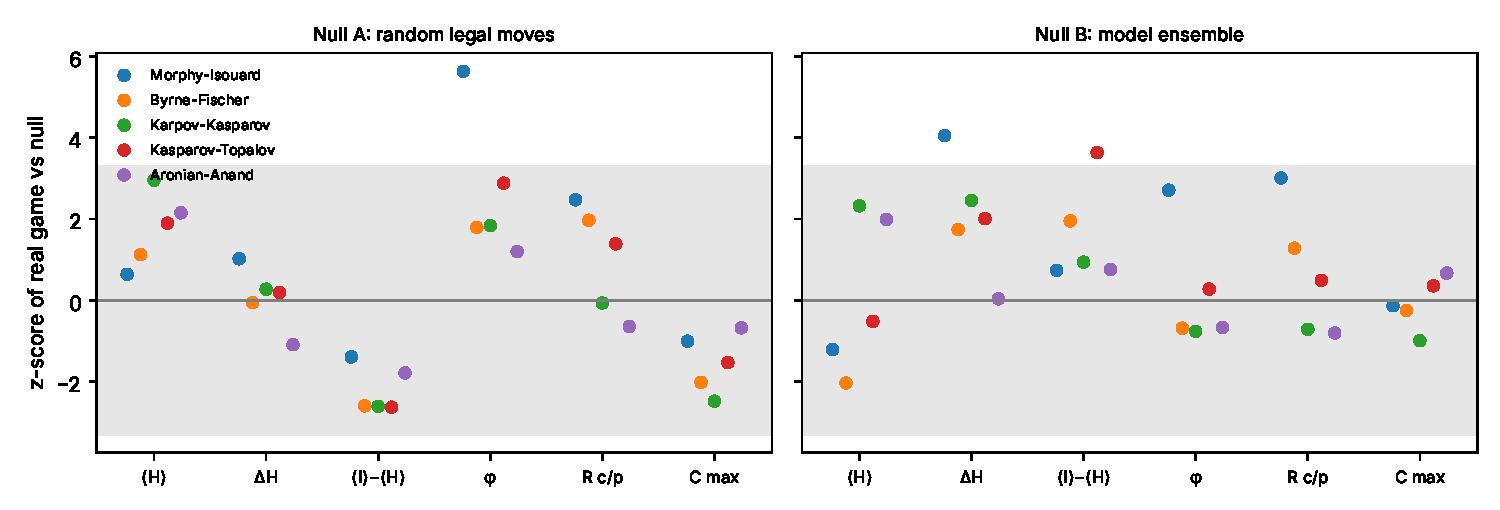
\includegraphics[width=\textwidth]{fig_z.pdf}
\caption{$z$-scores of the five real games against the two null ensembles for six observables. The shaded band marks $|z|<3.3$.}\label{fig:z}
\end{figure}

\subsection{Sensitivity to the ensemble temperature}
Table~\ref{tab:beta} repeats the entropy analysis at $\beta=0.5$, 1 and 2. The surprisal--entropy gap is negative at $\beta=0.5$ ($-0.18$ to $-0.28$ bits), small and positive at $\beta=1$ and large and positive at $\beta=2$ ($+1.25$ to $+1.68$ bits). The entropy drop $\Delta H$ grew with $\beta$ in every game except Byrne--Fischer, where it was nearly flat (1.37, 1.40, 1.44), and for Aronian--Anand it changed sign (from $-0.34$ at $\beta=0.5$ to $+2.37$ at $\beta=2$). The null ensembles were generated at $\beta=1$ only.

\begin{table}[t]
\centering
\caption{Sensitivity of the entropy observables to the inverse temperature $\beta$ (columns: $\beta=0.5$, 1, 2).}\label{tab:beta}
\resizebox{\textwidth}{!}{\begin{tabular}{lrrrrrrrrr}
\toprule
 & \multicolumn{3}{c}{$\langle H\rangle$ (bits)} & \multicolumn{3}{c}{$\Delta H$ (bits)} & \multicolumn{3}{c}{$\langle I\rangle-\langle H\rangle$ (bits)} \\
\cmidrule(lr){2-4}\cmidrule(lr){5-7}\cmidrule(lr){8-10}
Game & 0.5 & 1 & 2 & 0.5 & 1 & 2 & 0.5 & 1 & 2 \\
\midrule
Morphy--Isouard & 4.55 & 4.09 & 3.38 & 1.17 & 2.33 & 3.10 & -0.26 & 0.12 & 1.25 \\
Byrne--Fischer & 4.24 & 3.67 & 2.97 & 1.37 & 1.40 & 1.44 & -0.28 & 0.23 & 1.48 \\
Karpov--Kasparov & 4.98 & 4.53 & 3.65 & 0.71 & 1.71 & 2.70 & -0.25 & 0.11 & 1.46 \\
Kasparov--Topalov & 4.49 & 3.95 & 3.35 & 1.04 & 1.61 & 1.87 & -0.18 & 0.40 & 1.68 \\
Aronian--Anand & 5.06 & 4.67 & 3.65 & -0.34 & 0.40 & 2.37 & -0.20 & 0.11 & 1.67 \\
\bottomrule
\end{tabular}
}
\end{table}

\subsection{Outcome of the hypotheses}
Table~\ref{tab:hyp} states how each hypothesis fared.

\begin{table}[t]
\centering
\caption{Outcome of the pre-specified hypotheses.}\label{tab:hyp}
\small
\begin{tabular}{p{0.07\textwidth}p{0.16\textwidth}p{0.67\textwidth}}
\toprule
 & Verdict & Evidence \\
\midrule
H1 & Not supported & Peak capture availability occurred at 0.23--0.72 of game length with no common window; clustering was not tested formally. \\
H2 & Partly supported & $\Delta H>0$ in all five games at $\beta=1$, but about equally large in random play, and its sign for Aronian--Anand depends on $\beta$. Surprisal exceeded entropy most at the sacrifices of Morphy, Fischer and Kasparov (94th--100th percentile), less at Anand's. \\
H3 & Partly supported & $R_{\mathrm{c/p}}>1$ in all games (1.70--2.81) and higher in the three sharp games (2.58--2.81) than the two positional ones (1.70--2.09), but random and model-sampled games gave similar values (1.8--2.4). \\
H4 & Weakly supported & 3 of 60 comparisons exceed $|z|=3.3$; the most consistent difference is a smaller surprisal--entropy gap than in random play. \\
H5 & Not supported & Rank correlation $\rho=0.40$ ($n=5$, $p\approx0.5$); queens survived most and knights least. \\
\bottomrule
\end{tabular}
\end{table}

%--------------------------------------------------------------------
\section{Discussion}\label{sec:discussion}

\paragraph{What the model measures.} The framework turns a game record into a compact, interpretable set of observables, and these differ between games in sensible ways: the three sharp games have a higher control-to-piece ratio than the two positional ones, and the sacrificial moves of Morphy, Fischer and Kasparov stand out in surprisal. Both effects are what one would expect from experience, and we report them as consistency checks rather than discoveries.

\paragraph{Much of the structure is kinematic.} Random play shows monotone density loss, an entropy drop of 1.2--1.5 bits and a control field that is more active than the piece field. These features follow from the rules and from material leaving the board, since $N_t$ shrinks as pieces disappear. A statement such as ``decision entropy decays during a game'' therefore tells us about the lattice gas more than about the players. The comparison with model-sampled play is the more informative one, and there real games lose entropy faster in four of five cases at $\beta=1$. Table~\ref{tab:beta} shows that this conclusion depends on $\beta$.

\paragraph{The surprisal test is partly circular.} The heuristic energy penalises moving a piece onto an attacked square, and a sacrifice is exactly such a move. Its high surprisal therefore shows that the model flags moves that give up material, not that sacrifices are special in a physical sense. Telling a brilliant sacrifice from a blunder needs engine-based energies, which the model's structure allows but this study did not use.

\paragraph{Survival and outcome.} Surviving weight at the end predicted the winner in only two of five games. This is expected: the king has zero weight, so a mating attack is invisible to the weight measure, and Morphy's win leaves the winner with the lower surviving weight. Material is one of several conserved-like quantities, and king safety would need its own observable.

\paragraph{The annihilation convention.} A chess capture is asymmetric, since the capturing piece survives; our merge into one particle is a bookkeeping choice. We did not test a symmetric accounting in which the capturer is also charged part of the victim's weight, and we cannot say how much the reported values of $\varphi$ depend on the convention.

\paragraph{Limitations.} The study has five games chosen for fame, not drawn at random, so nothing here is a statement about chess in general. Move energies come from a simple heuristic, and the weights were fixed at conventional values with no sweep. The null ensembles used a single $\beta$. The $z$-scores come from distributions of 1000 games, so the extreme tail is only roughly resolved, and with 60 comparisons the $|z|\ge3.3$ marker is a rule of thumb, not a formal correction.

\paragraph{Transfer to other systems.} The pipeline needs only a record of which site was occupied by which species at each time, and which reactions occurred. Table~\ref{tab:map} gives proposed mappings. 

\begin{table}[t]
\centering
\caption{Proposed mappings of the model onto other domains (analogies, untested).}\label{tab:map}
\small
\begin{tabular}{p{0.16\textwidth}p{0.17\textwidth}p{0.16\textwidth}p{0.17\textwidth}p{0.22\textwidth}}
\toprule
Domain & Species & Exclusion & Reaction & Decision \\
\midrule
Reaction kinetics & Two reactants & One particle per site & $A+B\to0$ on contact & None (random walk) \\
Ecology & Two competing populations & One individual per patch & Fatal encounter & Foraging, movement \\
Order-book markets & Buy and sell orders & One order per price level & Order matching & Where and when to submit \\
Immunology & Pathogen and immune cells & One cell per binding site & Neutralisation & Which target to engage \\
Conflict & Opposing forces & One unit per location & Attrition & Commit or hold \\
\bottomrule
\end{tabular}
\end{table}
%--------------------------------------------------------------------
\section{Conclusion}\label{sec:conclusion}

Chess can be described as an annihilating Boolean lattice gas whose observables---density, immune fraction, surviving weight, Boolean activity, decision entropy and surprisal---are computed directly from a game record. On five verified classic games the framework gives consistent and interpretable output and flags sacrificial moves by their surprisal. At this stage, with heuristic move energies and five games, it does not show that real games differ strongly from random or model-sampled play: three of 60 comparisons were clearly outside the null, several apparent regularities are kinematic, and the entropy conclusions depend on the ensemble temperature. The value of the work for now is the measurement framework and the open tool, which are ready for engine-based energies and larger corpora, and for the first tests outside chess.

%--------------------------------------------------------------------
\section*{Data and code availability}\label{sec:data}
The software (\texttt{chess\_physics.py}), the study scripts for data verification, null ensembles and statistics, the verified PGN files, per-ply tables and figures are provided with this article. The move records were transcribed from the following pages (accessed 22 October 2026); in each pair the first source was used for analysis and the second for verification.

\begin{itemize}\setlength\itemsep{0pt}\small
\item Morphy, 1858: \url{https://en.wikipedia.org/wiki/Opera_Game}; \url{https://gameknot.com/annotation.pl/the-opera-game?gm=12022}
\item Byrne--Fischer, 1956: \url{https://en.wikipedia.org/wiki/Game_of_the_Century_(chess)}; \url{https://en.chessbase.com/news/2006/games/fischer1956g0.htm}
\item Karpov--Kasparov, 1985, game 16: \url{https://en.wikipedia.org/wiki/World_Chess_Championship_1985}; \url{https://chess.com/blog/ThummimS/world-chess-championship-1985-game-16-karpov-vs-kasparov}. A third record in descriptive notation (\url{https://csmonitor.com/1985/1106/lchs06.html}) agrees in length and result but was not machine-compared.
\item Kasparov--Topalov, 1999: \url{https://en.wikipedia.org/wiki/Kasparov\%27s_Immortal}; \url{https://chess.com/blog/Eshwar360/the-best-chess-game-of-all-time-garry-kasparov-vs-veselin-topalov-1999}
\item Aronian--Anand, 2013: \url{https://en.wikipedia.org/wiki/Anand\%27s_Immortal}; \url{https://en.chessbase.com/home/TabId/211/PostId/4008776}
\end{itemize}


\section*{Competing interests}
The author declares no competing interests.

%--------------------------------------------------------------------
\bibliographystyle{unsrtnat}
\bibliography{refs}

\end{document}
